% CONTEXT_REPORT_STATUS: final
\section{上下文预算与 QA 收尾消融（11月1日）}
\label{sec:context-optimization}
本节保留11月1日的实验、评分及当时的验证记录；11月2日的追加实验另列，不择高拼接不同批次分数。
本节固定已生成的多模态记忆，仅重新运行 QA。旧 oGMemory 和 M3-Agent 为固定的既有答案；A/B/C/D及B的完整重复均保留，未择高。将七组共455条答案交错打乱后用相同 MiniMax 评委重新评分，评委不接收方案名称。初次评分仍保留；共同重评批次与前节不同，旧答案本身没有修改。
\begin{center}\small
\begin{tabular}{lrrrrrr}\toprule
方案 & 有效回答 & 独立评分 & 共同评分 & 输入/M & 峰值/k & 调用\\\midrule
原固定答案 & 59/65 & 0.5462 & 0.5385 & 19.906 & 156.69 & 319\\
M3参考协议 & 65/65 & 0.4615 & 0.4615 & 0.570 & 4.74 & 310\\
A：仅预算 & 65/65 & 0.5538 & 0.5538 & 4.722 & 16.90 & 359\\
B：预算+收尾 & 65/65 & 0.6000 & 0.6077 & 4.804 & 16.92 & 365\\
C：12k+收尾 & 64/65 & 0.5231 & 0.5231 & 2.722 & 9.10 & 366\\
D：12k分组+收尾 & 65/65 & 0.5308 & 0.5385 & 2.760 & 9.25 & 366\\
B独立重复 & 65/65 & 0.5615 & 0.5769 & 4.708 & 16.93 & 361\\
\bottomrule\end{tabular}\end{center}
A曾遇到套餐额度中断：恢复时保留55条成功答案和48条成功评分，只补做额度导致的失败与未评分部分。B的前次尝试没有有效答案，另立目录完整运行。原失败记录和未知usage的请求开销均保留，未按题挑选高分。
评分为0、0.5、1自动评分的全65题均值，不是人工准确率。输入包含缓存tokens，不等于费用；跨时段服务负载不同，不能据此声称严格墙钟加速比。
五组新轨迹共325条QA记录，324条有效回答，记录到0条QA超时；单题实际墙钟最大112.53秒。这些是恢复后的固定轨迹，先前额度失败另列。C的一条协议校验失败保留计零；没有把done状态直接当作有效答案。
\subsection{逐视频共同评分}
\begin{center}\small\begin{tabular}{lrrrrrrr}\toprule
视频 & 原答案 & M3参考 & A & B & C & D & B重复\\\midrule
study\_05 & 0.3333 & 0.5417 & 0.5000 & 0.6250 & 0.5417 & 0.2917 & 0.5000\\
gym\_03 & 0.7273 & 0.5455 & 0.6364 & 0.7273 & 0.6818 & 0.7727 & 0.6818\\
bedroom\_04 & 0.6364 & 0.6364 & 0.8182 & 0.8182 & 0.6364 & 0.8182 & 0.8182\\
study\_18 & 0.3214 & 0.2500 & 0.2857 & 0.3214 & 0.2500 & 0.2857 & 0.2500\\
kitchen\_20 & 0.6765 & 0.4118 & 0.5882 & 0.6176 & 0.5588 & 0.5882 & 0.6765\\
\bottomrule\end{tabular}\end{center}
\subsection{诊断、机制与限制}
原6道超时题的模型调用累计183--230秒，检索仅1.1--1.7秒。首轮约1250输入tokens，随后重复的完整片段对象使输入累积至9万--12万。A复用原仓已有但正式基线未开启的上下文预算模块：内容版本去重、连续原文选择、有效引用和完整请求计数。22528输入预算预留8192输出及2048安全空间。新组还统一限制请求top-k不超过16、候选不超过32、单次总返回节点不超过24、每题Search尝试不超过8次；A因此是整套有界策略，而不只是删除重复字符串。B增加45秒回答预留，并在最后一轮关闭Search；C将输入估计上限降为12000。D在相同12000预算下将已选原文按字段分组，去除重复包装和模型无需读取的内容哈希；原始值、来源范围、人物与时间元数据不改写，完整哈希保留在审计中。计数器使用本地Qwen tokenizer代理，不等同于MiniMax的精确模板。

A：仅预算相对原答案评分差为+0.0154，累计输入下降76.3\%，峰值下降89.2\%。按5个完整视频簇枚举重采样的95\%区间为[-0.0786, +0.1250]。

B：预算+收尾相对原答案评分差为+0.0692，累计输入下降75.9\%，峰值下降89.2\%。按5个完整视频簇枚举重采样的95\%区间为[-0.0286, +0.2049]。

C：12k+收尾相对原答案评分差为-0.0154，累计输入下降86.3\%，峰值下降94.2\%。按5个完整视频簇枚举重采样的95\%区间为[-0.0921, +0.1066]。

D：12k分组+收尾相对原答案评分差为+0.0000，累计输入下降86.1\%，峰值下降94.1\%。按5个完整视频簇枚举重采样的95\%区间为[-0.0625, +0.1000]。

B独立重复相对原答案评分差为+0.0385，累计输入下降76.4\%，峰值下降89.2\%。按5个完整视频簇枚举重采样的95\%区间为[-0.0448, +0.1316]。

5/5个方案或重复运行的上述区间包含0。这些仅是五个开发视频的探索性重采样结果，不能据此宣称稳定的统计显著质量增益。
\subsection{覆盖恢复与已有答案的取舍}
主指标仍使用全65题。以下仅将总分变化分解为原59道有答案题与原6道无答案题的贡献，不改用成功子集均分，也不把这一记账分解当成单一因素的因果证明。
\begin{center}\small\begin{tabular}{lrrr}\toprule
条件 & 原59题分值变化 & 原6题分值变化 & 净分值变化\\\midrule
A：仅预算 & -4.0 & +5.0 & +1.0\\
B：预算+收尾 & -1.5 & +6.0 & +4.5\\
C：12k+收尾 & -6.0 & +5.0 & -1.0\\
D：12k分组+收尾 & -4.0 & +4.0 & +0.0\\
B独立重复 & -2.5 & +5.0 & +2.5\\
\bottomrule\end{tabular}\end{center}
本批总分进展主要伴随原超时题恢复，原已回答题仍有损失。因此结论是效率与回答覆盖得到改善，但单题事实质量存在取舍，不能声称推理能力普遍提升。
\subsection{重复运行与评分波动}
B两次共同评分为0.6077与0.5769，绝对差0.0308；12题的自动评分不同。两轮均分的描述性平均为0.5923，不择高、不拼接答案。同一65题的重复不等于130个独立新问题，仅两轮不能精确估计随机波动或支持泛化结论。
上述区间仅用于呈现小样本不确定性：五个视频均为开发样本，不是独立留出集。未触发时间预留的运行不能证明45秒机制带来收益；提前收尾也不能保证单个极慢HTTP不会越过软截止。M3-Agent仍为同模型适配而非官方权重复现。原文被预算省略不等于事实不存在，计数题尤其不能把入选片段数当作真实次数。
源帧定性检查还发现：study\_18第14片段的输入止于435秒远景，445--446秒出现的货架近景与取纸动作没有进入16帧前缀采样。这提示采帧/记忆细节的上游限制，但这些尾段帧在434秒问题时间之后，只在本次current\_clip宽限内，不能用于严格因果评测。辅助检查没有改变任何本轮模型输入或答案。
详细结果、逐题变化和验证记录位于\path{experiments/m3_context_study_20261101/}；设计说明见\path{docs/m3_context_optimization.md}。
\subsection{缓存与未缓存输入}
\begin{figure}[htbp]\centering
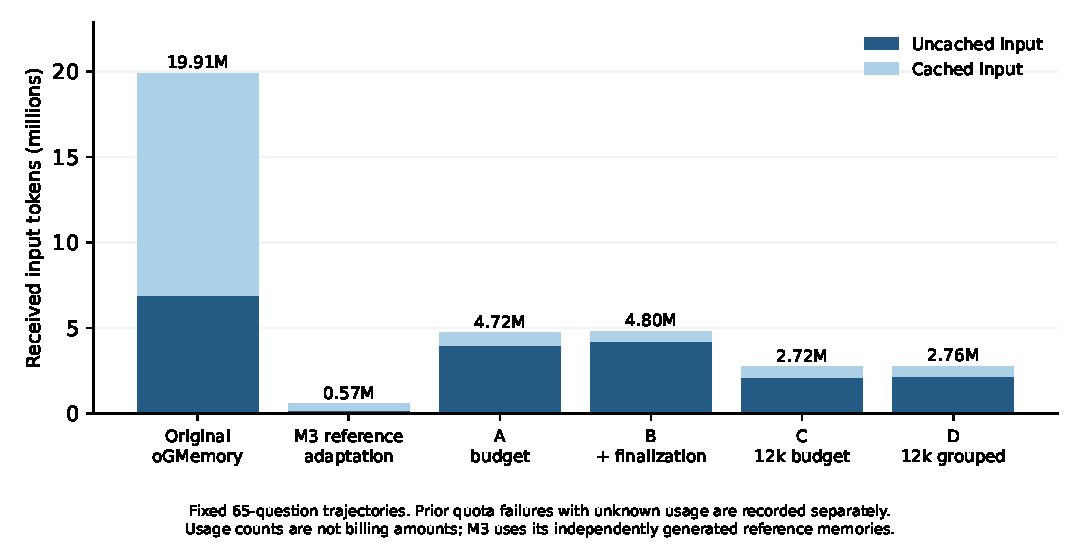
\includegraphics[width=\linewidth]{figures/context_cache.pdf}
\caption{固定答案轨迹的实际输入用量。深色为未缓存输入，浅色为缓存输入；未知usage的额度失败请求另行保留，不计作零费用。}\end{figure}
重打包会改变较早的工具消息，可能削弱稳定前缀。实际usage显示缓存比例改变，因此总输入降幅不能直接当成费用或套餐额度降幅。缓存内部实现与跨时段服务负载没有被本实验严格控制。
相同12000预算下，D最终视图平均保留78.83条原文条目/片段，C为66.66。这不是独立事实计数；查询轨迹也不同，不能解读为固定查询的信息增益。压缩空间可能用于装入更多原文而非降低API输入，是否有助于答案质量仍需看实际评测。
本轮所有实际调用日志去除重复文件后共记录2635次逻辑调用，45次usage未知；收到输入20.202M和输出0.497M tokens，另有209-token可用性探针。此为全部试验开销，与单条件固定轨迹用量不同；不含先前记忆生成与历史基线，也不是账单。强制停止时未落盘的在途请求无法凭现有日志完整计量。
\subsection{验证与配置使用}
当前发布代码的M3/provider/core单元检查1041项通过；扩大检查排除9项已复现的既有问题后为1388通过、108跳过、9排除。不能将排除等同于修复，也不能称整个仓库全部通过。各实验使用各自冻结源码，源码文件与Git归档逐项核对；共同评分输入和原预测文件在发布前重新校验，而不只信任状态标记。
可用\code{python -m m3.configure_qa_context}生成新的0600配置副本，保留模型与连接设置。它针对ReAct QA/pipeline，不是旧单次QA入口；切换策略必须使用新的输出目录，不应跨配置resume旧答案。
\subsection{本轮建议}
质量优先时建议先采用balanced：输入目标24000，在8192输出和2048安全预留下实际输入估计上限为22528，6轮/180秒，并保留终轮Answer-only与控制提示。45秒预留本轮未实际触发，仅能作为经单元验证的保护机制。compact/grouped保持可选，不因编码更短或原文更多就默认上线。
下一阶段应在新视频及严格时间策略下验证前缀更稳定的证据交付、带来源与可用时间的实体事实索引；采帧覆盖、身份归属和事件计数应单独消融，不能通过引入未来帧或事后答案改变本轮成绩。
